Designed modeling tools mentioned earlier include the quantitative model of
utilization of allocation time and the simulator of jobs processing at a
supercomputer.

The quantitative model allows to calculate a probability of achieving
required utilization of allocated resources in a given time by defining
specific parameters for jobs processing. Some of these parameters are set by
the user (e.g., the number of requested nodes and walltime), while other
parameters are determined by a particular workload of a supercomputer and
actions (i.e., activity) of other users (e.g., the waiting time of the job
in the supercomputer's queue before it runs on computing nodes). The basic
version of the model assumes that jobs, which utilization is under the
estimation, are launched sequentially: every next job arrives to the
supercomputer queue only after the previous job has been started to run on
computing nodes.

Equation that describes the quantitative model (its derivation process is
presented in the Appendix~\ref{appendix-model-derivation}):
\begin{equation}
    \label{eq-quantitative-model}
    \begin{multlined}
    P(U > U_0) = \sum\limits_{n=100}^{\infty} 
                 \bigg[
                 \int_{U_0}^{\infty}f(x, n\mu_{U}, n\sigma_{U}^2)dx \
                 \times \\
                 \bigg( \int_{-\infty}^{T_0}f(x, n\mu, n\sigma^2)dx \  - \\
                 \int_{-\infty}^{T_0}f(x, (n+1)\mu, (n+1)\sigma^2)dx \bigg)
                 \bigg]
    \end{multlined}
\end{equation}

The outcome of the Equation~\ref{eq-quantitative-model} is the probability
that the utilization of resources, which is achieved by a sequential set of
processed jobs using capabilities of the supercomputer during the time
interval $T_0$, is greater than the predefined value $U_0$. It implies that:
\begin{itemize}
    \item Utilization of every single job is described by a random variable
    with the expected value $\mu_{U}$ and the variance $\sigma_{U}^2$;
    \item The time interval between launches of sequential jobs is described
    by a random variable with the expected value $\mu$ and the
    variance $\sigma^2$.
\end{itemize}

Another modeling tool is the simulator which is aimed to simulate the workload
on a supercomputer and to produce job traces for a given workload, as well,
it is used for the quantitative model validation and adjustment. There are
two modes to run the simulator: i) set operational parameters, such as job
generation rate and job execution rate, to produce synthetic data only; ii)
use historical data for key parameters of a job, such as timestamp of job
arrival to the queue and job execution time, to produce simulated data of
real job processing life-cycle.

The simulator is based on Queueing Theory~\cite{ref-queueing-theory} and
according to the Kendall's Notation~\cite{ref-kendall} for queues, usually
referred as A/B/C/D/E, it is characterized as following:
\begin{itemize}
    \item A - \textit{arrival process} is represented by streams that are
    responsible for job generation and is described either by a Poisson
    process or by a deterministic model;
     \item B - \textit{service/server process} is represented by a set of
    nodes that simulate job execution process and is described either by a
    Poisson process or by a deterministic model as well;
    \item C - \textit{number of servers} that corresponds to the number of
    computing nodes (in terms of the Titan supercomputer);
    \item D - \textit{capacity of the queue or system overall}, which is
    ``on'', if the queue limit is set (either per stream or for the total
    number of jobs in the queue) and queue buffer is not used, otherwise the
    capacity is unlimited;
    \item E - \textit{queueing discipline} is provided in two options: FIFO
    or Priority.
\end{itemize}

Some of the parameters are set as requirements and restrictions applied to a
specific supercomputer and its policy, e.g., the total number of computing
nodes that are available for computing jobs, the limit of the number of jobs
in the queue per user/group, etc.

\subsubsection{Simulator description} \label{sec-strategy-2-1}

Implementation of the simulator (Queueing System Simulator) \cite{ref-qss}
was done by using Python\footnote{High-level programming language Python,
\url{https://docs.python.org/2.7/} [accessed on 2020-01-10]}, and the
following key classes and generators were designed (to emulate internal
supercomputer processes):
\begin{itemize}
    \item \textit{Job} - contains parameters to describe job's processing
    life-cycle, such as arrival timestamp, start execution timestamp,
    completion timestamp that is based on walltime / execution time along
    with the previous parameter, number of required nodes for its execution,
    stream (i.e., source name), label (i.e., project name), priority and
    priority group name;
    \item \textit{Stream} - generates jobs with the predefined parameters as
    an input for the simulator;
    \item \textit{Queue Manager} - emulates buffer ahead of the queue, the
    queue itself, and manages jobs while waiting for their execution, it
    lets to define the queue discipline such as FIFO and Priority, and set
    the limits per input job stream;
    \item \textit{Schedule Manager} - emulates a backfill mode - gets
    information about job sizes, assigns corresponding nodes for execution,
    gives a schedule when each job starts to be executed;
    \item \textit{QSS} - the core class that manages and tracks job's
    processing life-cycle.
\end{itemize}

\subsubsection{State model} \label{sec-strategy-2-2}

Job life-cycle (in terms of the simulator,
Figure~\ref{fig-simulator-scheme}) includes the following states:
\textbf{Generated} - \textbf{Holding} (i.e., Titan notation: blocked)
[buffer] - \textbf{Pending} (i.e., Titan notation: eligible-to-run) [queue] -
\textbf{Starting} - \textbf{Executing} - \textbf{Finished}. Some of the
states might be skipped if certain components are turned off (e.g., if the
queue buffer is not used then there is no state ``holding'') or if there is
some initial restriction (e.g., state ``starting'' is neglected, since the
assumption that job execution starts right after it leaves the queue).

\begin{figure}
    \centering
    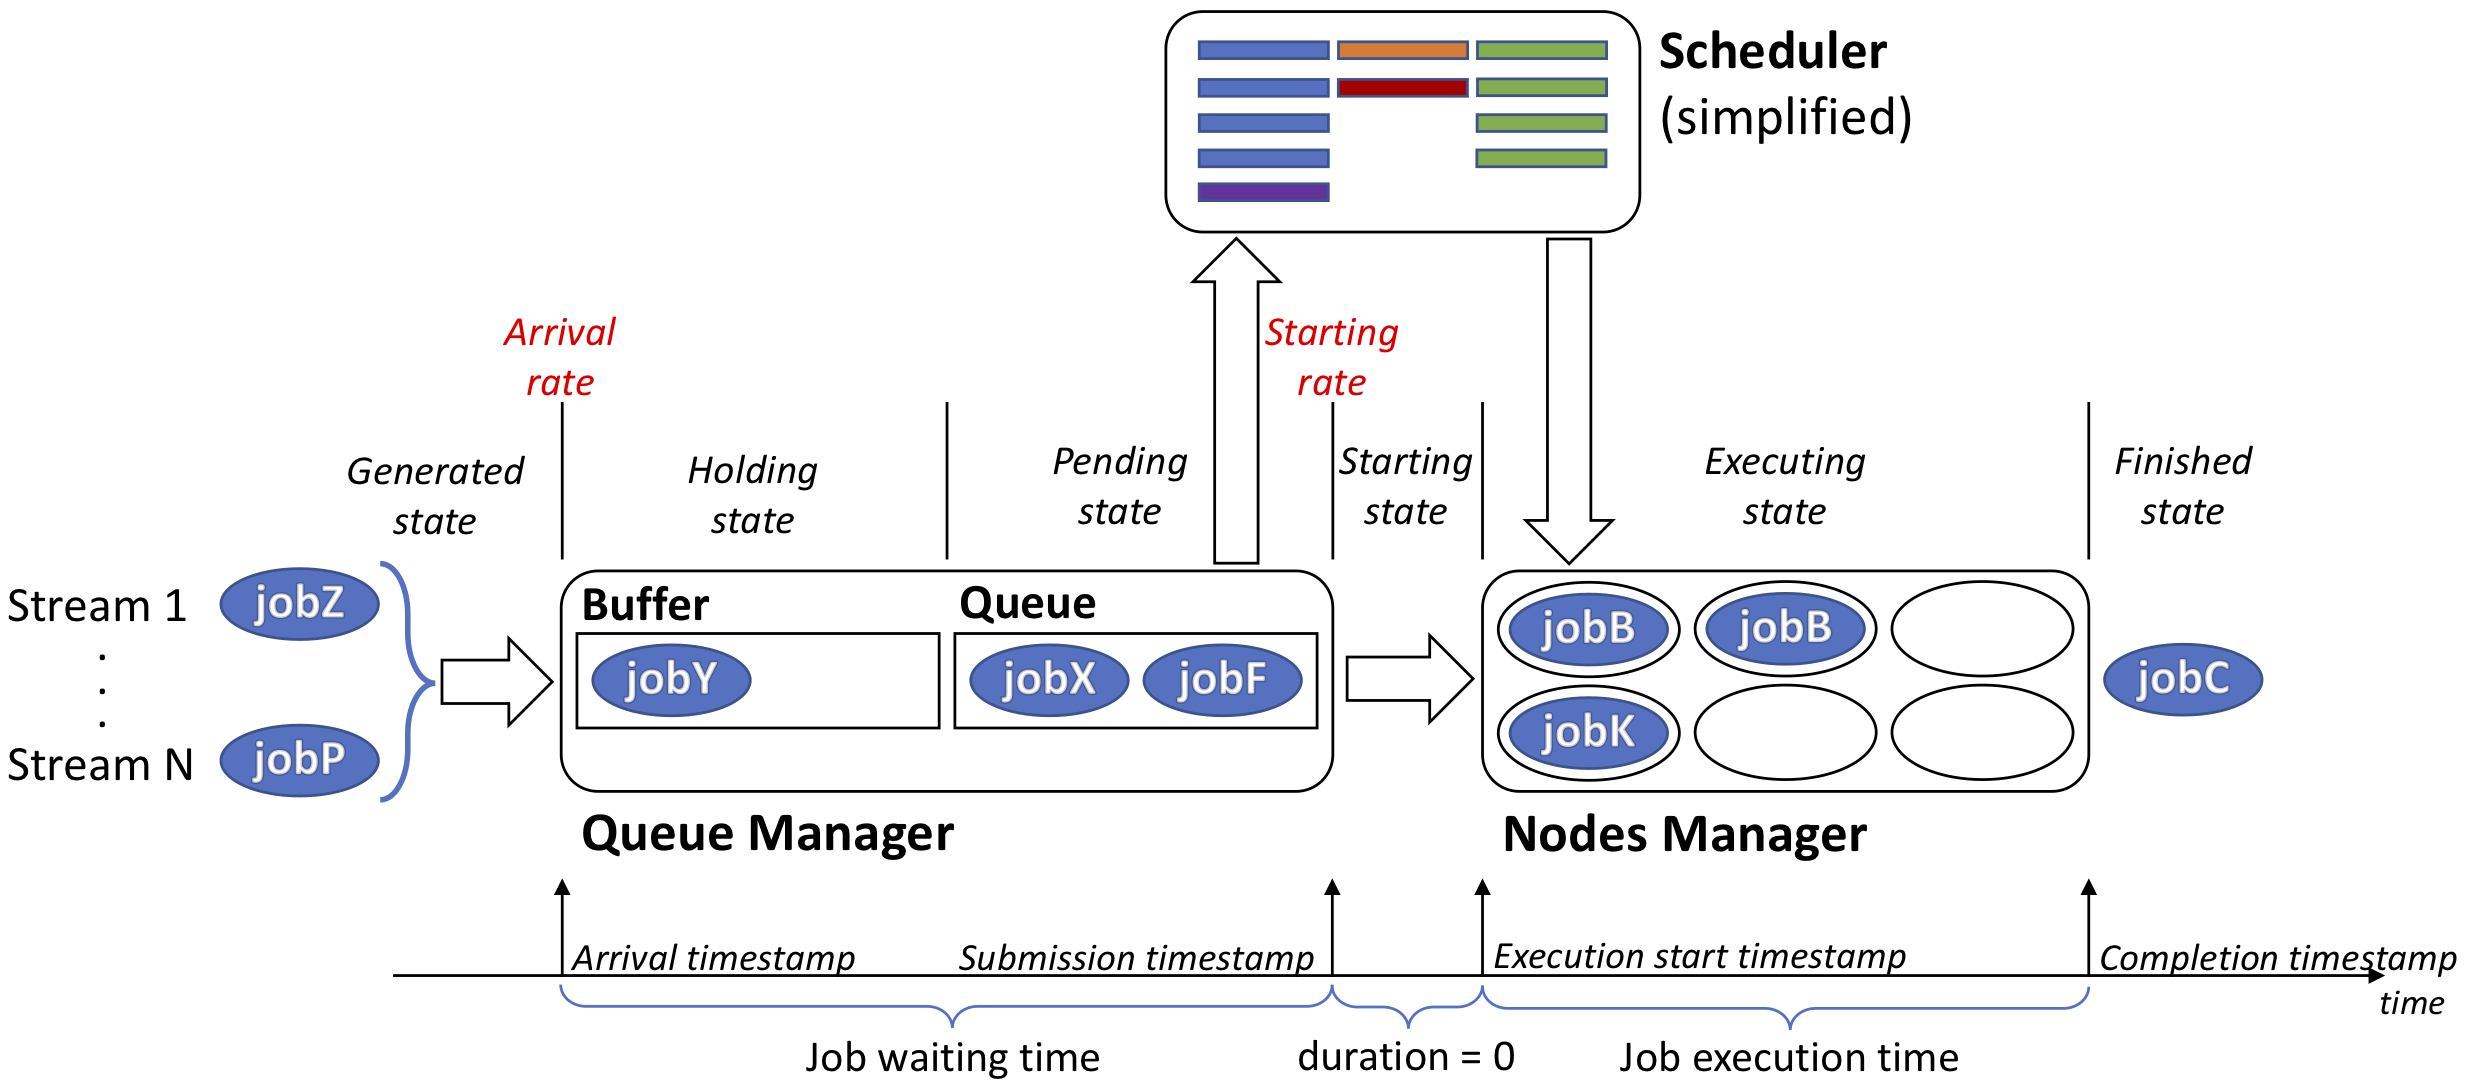
\includegraphics[width=0.48\textwidth]{pics/simulator-scheme.png}
    \caption{Job state transitions at the simulator}
    \label{fig-simulator-scheme} 
\end{figure}
